\section{第1讲\quad 空间几何体}
\subsection{夯基础}
\bktopic{构成空间几何体的基本元素及其关系}

\begin{example}[\bkstar{1}{5}]
如图中，点、直线、平面之间的关系用集合语言可表示为
\bkfig{TikZ-final/geometry/solid/p004-o0099.tex}
\begin{tasks}(1)
    \task $\alpha\cap\beta=m$，$n\subset\alpha$，$m\cap n=A$
    \task $\alpha\cap\beta=m$，$n\in\alpha$，$m\cap n=A$
    \task $\alpha\cap\beta=m$，$n\subset\alpha$，$A\subset m$，$A\subset n$
    \task $\alpha\cap\beta=m$，$n\in\alpha$，$A\in m$，$A\in n$
\end{tasks}
\end{example}
\begin{solution}
\textbf{答案：}A

由已知可得如图
\bkfig{TikZ-final/geometry/solid/p046-o0974.tex}
由图可知 $A$ 为点，$n$ 为直线，故可得 $n\subset\alpha$，则 $n\in\alpha$ 表示不正确，故排除B，D，而 $A\subset m$，$A\subset n$ 也表述不正确，故排除C，则A正确．

故选：A．
\end{solution}

\vspace{2em}

\bktopic{空间划分问题}

\begin{example}[\bkstar{2}{5}]
三个平面将空间最多能分成
\begin{tasks}(4)
    \task $6$ 部分
    \task $7$ 部分
    \task $8$ 部分
    \task $9$ 部分
\end{tasks}
\end{example}
\begin{solution}
\textbf{答案：}C

三个平面两两平行时，可以把空间分成 $4$ 部分；三个平面相交于同一条直线时，可以把空间分成 $6$ 部分；两个平面平行，第三个平面与它们相交时，可以把空间分成 $6$ 部分；三个平面两个相交，且交线互相平行时，可以把空间分成 $7$ 部分；三个平面两两相交，当三条不同的交线相交于一点时，可以把空间分成 $8$ 部分．所以空间中的三个平面最多能把空间分成 $8$ 部分．

故选：C．
\end{solution}

\vspace{2em}

\bktopic{棱锥的结构特征}

\begin{example}[\bkstar{2}{5}]
如图所示，观察四个几何体，其中判断正确的是
\begin{tasks}(4)
    \task \raisebox{-.5\height}{\resizebox{0.12\textwidth}{!}{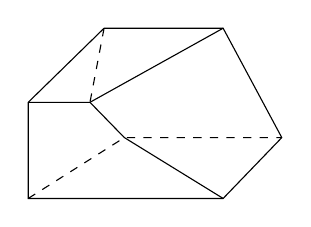
\begin{tikzpicture}[scale=.56]
  \coordinate (A) at (0,0); \coordinate (B) at (0,2.18);
  \coordinate (C) at (1.40,2.18); \coordinate (D) at (2.18,1.38);
  \coordinate (E) at (1.72,3.86); \coordinate (F) at (4.42,3.86);
  \coordinate (G) at (5.75,1.38); \coordinate (H) at (4.42,0);
  \draw (A)--(B)--(E)--(F)--(G)--(H)--cycle;
  \draw (B)--(C)--(D)--(H);
  \draw (C)--(F);
  \draw[dashed] (E)--(C) (A)--(D)--(G);
\end{tikzpicture}
}}\ 是棱台
    \task \raisebox{-.5\height}{\resizebox{0.08\textwidth}{!}{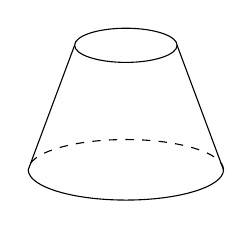
\begin{tikzpicture}[scale=.62]
  \draw (0,2.55) ellipse (1.05 and .35);
  \draw (-2,0) -- (-1.05,2.55) (2,0) -- (1.05,2.55);
  \draw (-2,0) arc[start angle=180,end angle=360,x radius=2,y radius=.62];
  \draw[dashed] (2,0) arc[start angle=0,end angle=180,x radius=2,y radius=.62];
\end{tikzpicture}
}}\ 是圆台
    \task \raisebox{-.5\height}{\resizebox{0.1\textwidth}{!}{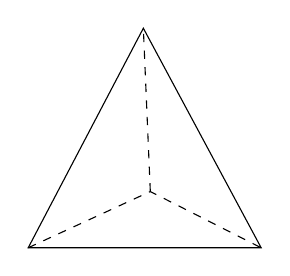
\begin{tikzpicture}[scale=.68]
  \coordinate (A) at (0,0); \coordinate (B) at (4.35,0);
  \coordinate (C) at (2.28,1.05); \coordinate (P) at (2.15,4.10);
  \draw (P)--(A)--(B)--cycle;
  \draw[dashed] (A)--(C)--(B) (C)--(P);
\end{tikzpicture}
}}\ 是棱锥
    \task \raisebox{-.5\height}{\resizebox{0.12\textwidth}{!}{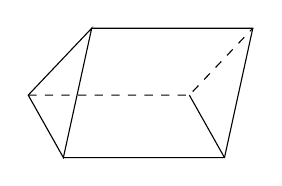
\begin{tikzpicture}[scale=.62]
  \coordinate (A) at (0,1.28); \coordinate (B) at (1.30,2.65);
  \coordinate (C) at (.72,0); \coordinate (D) at (3.30,1.28);
  \coordinate (E) at (4.60,2.65); \coordinate (F) at (4.02,0);
  \draw (A)--(B)--(C)--cycle;
  \draw (B)--(E)--(F)--(C);
  \draw (D)--(F);
  \draw[dashed] (A)--(D)--(E);
\end{tikzpicture}
}}\ 不是棱柱
\end{tasks}
\end{example}
\begin{solution}
\textbf{答案：}C

A．不满足棱台的定义，不正确；

B．不满足圆台的定义，不正确；

C．是棱锥，正确；

D．是棱柱，不正确．

故选：C．
\end{solution}

\vspace{2em}

\begin{example}[\bkstar{2}{5}]
将一个直角梯形绕其较短的底所在的直线旋转一周得到一个几何体，关于该几何体的以下描绘中，正确的是
\begin{tasks}(2)
    \task 是一个圆台
    \task 是一个圆柱
    \task 是一个圆柱和一个圆锥的简单组合体
    \task 是一个圆柱被挖去一个圆锥后所剩的几何体
\end{tasks}
\end{example}
\begin{solution}
\textbf{答案：}D

将一个直角梯形绕其较短的底所在的直线旋转一周得到一个圆柱被挖去一个圆锥后所剩的几何体．

故选：D．
\end{solution}

\vspace{2em}

\bktopic{多面体中的基础计算}

\begin{example}[\bkstar{2}{5}]
一个长方体的长、宽、高分别为 $3$，$4$，$5$，则这个长方体的体对角线长是
\begin{tasks}(4)
    \task $12$
    \task $10$
    \task $5\sqrt{2}$
    \task $2\sqrt{5}$
\end{tasks}
\end{example}
\begin{solution}
\textbf{答案：}C

由题意，长方体的体对角线长是 $\sqrt{9+16+25}=5\sqrt{2}$．

故选：C．
\end{solution}

\vspace{2em}

\begin{example}[\bkstar{2}{5}]
已知正四棱锥的底面边长为 $6$，高为 $4$，则斜高为
\begin{tasks}(4)
    \task $4$
    \task $3\sqrt{2}$
    \task $5$
    \task $4\sqrt{2}$
\end{tasks}
\end{example}
\begin{solution}
\textbf{答案：}C

如图
\bkfig[0.35\textwidth]{TikZ-final/geometry/solid/p047-o0996.tex}
$\because$ 正四棱锥 $P-ABCD$ 的底面边长为 $6$，$E$ 为 $AD$ 的中点，$O$ 为底面正方形的中心，

$\therefore OE=3$．

又正四棱锥的高 $PO=4$，所以斜高

$$
PE=\sqrt{PO^2+OE^2}=\sqrt{16+9}=5．
$$

故选：C．
\end{solution}

\vspace{2em}

\bktopic{表面积与体积}

\begin{example}[\bkstar{2}{5}]
一个高为 $2$ 的圆柱，底面周长为 $2\pi$，该圆柱的表面积为
\end{example}
\begin{solution}
\textbf{答案：}$6\pi$

因为一个高为 $2$ 的圆柱，底面周长为 $2\pi$，所以它的底面半径为 $1$，所以圆柱的表面积为

$$
S=2S_{\text{底}}+S_{\text{侧}}=2\times 1^2\times\pi+2\pi\times 2=6\pi．
$$

故答案为：$6\pi$．
\end{solution}

\vspace{2em}

\begin{example}[\bkstar{2}{5}]
圆锥的底面半径为 $1$，高为 $\sqrt{3}$，则圆锥的表面积为
\begin{tasks}(4)
    \task $\pi$
    \task $2\pi$
    \task $3\pi$
    \task $4\pi$
\end{tasks}
\end{example}
\begin{solution}
\textbf{答案：}C

圆锥的底面半径为 $1$，高为 $\sqrt{3}$，则母线长 $l=\sqrt{1^2+\left(\sqrt{3}\right)^2}=2$，圆锥的表面积

$$
S=S_{\text{底面}}+S_{\text{侧面}}=\pi r^2+\pi rl=\pi+2\pi=3\pi．
$$

故选：C．
\end{solution}

\vspace{2em}

\bktopic{球}

\begin{example}[\bkstar{2}{5}]
半径为 $2$ 的球的表面积为
\begin{tasks}(4)
    \task $4\pi$
    \task $8\pi$
    \task $12\pi$
    \task $16\pi$
\end{tasks}
\end{example}
\begin{solution}
\textbf{答案：}D

$\because$ 球的半径 $R=2$，

$\therefore$ 球的表面积为 $4\pi\times R^2=4\pi\times 4=16\pi$．

故选：D．
\end{solution}

\vspace{2em}

\begin{example}[\bkstar{1}{5}]
已知球的半径为 $1$，则该球的体积是
\begin{tasks}(4)
    \task $\dfrac{4}{3}$
    \task $\pi$
    \task $\dfrac{4\pi}{3}$
    \task $4\pi$
\end{tasks}
\end{example}
\begin{solution}
\textbf{答案：}C

由球的体积公式得 $V=\dfrac{4\pi}{3}$．

故选：C．
\end{solution}

\vspace{2em}

\subsection{刷中档}
\bktopic{棱锥的结构特征}

\begin{example}[\bkstar{2}{5}]
若一个棱锥的各棱长均相等，则该棱锥一定不是
\begin{tasks}(4)
    \task 三棱锥
    \task 四棱锥
    \task 五棱锥
    \task 六棱锥
\end{tasks}
\end{example}
\begin{solution}
\textbf{答案：}D

若一个棱锥的各棱长均相等，则该棱锥一定不是六棱锥．因为正六边形的顶点到中心的距离等于边长，所以正六棱锥的侧棱必大于底面棱长．

故选：D．
\end{solution}

\vspace{2em}

\begin{example}[\bkstar{2}{5}]
某人用如图所示的纸片，沿折痕折后粘成一个四棱锥形的“走马灯”，正方形做灯底，且有一个三角形面上写上了“福”字，当灯逆时针旋转时，正好看到“幸福芜湖”的字样，则在①②③处可以依次写上
\bkfig[0.2\textwidth]{TikZ-final/geometry/solid/p006-o0134.tex}
\begin{tasks}(1)
    \task 芜、幸、湖
    \task 湖、幸、芜
    \task 幸、芜、湖
    \task 湖、芜、幸
\end{tasks}
\end{example}
\begin{solution}
\textbf{答案：}C

画出图形，如图所示．
\bkfig[0.3\textwidth]{TikZ-final/geometry/solid/p049-o1025.tex}
根据四棱锥图形，正好看到“幸福芜湖”的字样，可知顺序为①福②③，则在①②③处可以依次写上幸、芜、湖．

故选：C．
\end{solution}

\vspace{2em}

\begin{example}[\bkstar{2}{5}]
下列各图都是正方体的表面展开图，将其还原成正方体后，所得正方体完全一致（数码相对位置相同）的是
\bkfig[0.6\textwidth]{TikZ-final/geometry/solid/p007-o0147.tex}
\begin{tasks}(4)
    \task （Ⅰ）和（Ⅳ）
    \task （Ⅰ）和（Ⅲ）
    \task （Ⅱ）和（Ⅲ）
    \task （Ⅱ）和（Ⅳ）
\end{tasks}
\end{example}
\begin{solution}
\textbf{答案：}B

（Ⅰ）图还原后，①④对面，②⑤对面，③⑥对面；

（Ⅱ）图还原后，①⑥对面，②⑤对面，③④对面；

（Ⅲ）图还原后，①④对面，②⑤对面，③⑥对面；

（Ⅳ）图还原后，①⑤对面，②④对面，③⑥对面．

综上，可得还原成正方体后，其中两个完全一样的是（Ⅰ）和（Ⅲ）．

故选：B．
\end{solution}

\vspace{2em}

\begin{example}[\bkstar{3}{5}]
正方体的直观图如图所示，则其展开图是（要求把可能的序号都填上）．
\bkfig[0.45\textwidth]{TikZ-final/geometry/solid/p007-o0148.tex}
\end{example}
\begin{solution}
\textbf{答案：}(4)

根据题意，可得：

对于（1），展开图中的上下两边的正方形的对边中点连线应该呈左右方向显现，故（1）的图形不符合题意；

对于（2），展开图中最右边的“日”字形正方形的对边中点连线应该是上下方向呈现，且应该在含有圆形的正方形的左边放置，故（2）的图形不符合题意；

对于（3），展开图中最右边的正方形应该与含有圆形的正方形相邻，故（3）的图形不符合题意；

对于（4），沿如图的红线将正方体的侧面剪裁，展开可得如（4）图的形状，故（4）的图形符合题意．
\bkfig{TikZ-final/geometry/solid/p050-o1038.tex}
故答案为：（4）．
\end{solution}

\vspace{2em}

\bktopic{表面积与体积}

\begin{example}[\bkstar{3}{5}]
如图所示，三棱柱 $ABC-A_1B_1C_1$ 的体积为 $6$．$O$ 为四边形 $BCC_1B_1$ 的中心，则四面体 $A_1-B_1OB$ 的体积为
\bkfig[0.3\textwidth]{TikZ-final/geometry/solid/p007-o0153.tex}
\end{example}
\begin{solution}
\textbf{答案：}$1$

如图，连接 $A_1C$，$B_1C$．
\bkfig[0.3\textwidth]{TikZ-final/geometry/solid/p050-o1043.tex}
在三棱柱 $ABC-A_1B_1C_1$ 中，$V_{A_1-BB_1C}=V_{A_1-B_1C_1C}$，而 $V_{A_1-BB_1C}=V_{C-A_1B_1B}=V_{C-AA_1B}$，

$\therefore$ 四面体 $A_1-B_1BC$ 的体积 $V=\dfrac{1}{3}V_{ABC-A_1B_1C_1}=\dfrac{1}{3}\times 6=2$，

则四面体 $A_1-B_1OB$ 的体积为 $\dfrac{1}{2}V_{A_1-BB_1C}=\dfrac{1}{2}\times 2=1$．

故答案为：$1$．
\end{solution}

\vspace{2em}

\begin{example}[\bkstar{2}{5}]
设三棱锥 $P-ABC$ 的三条侧棱两两垂直，且满足 $PA=PB=PC=1$，则三棱锥 $P-ABC$ 的体积是
\end{example}
\begin{solution}
\textbf{答案：}$\dfrac{1}{6}$

因为三棱锥 $P-ABC$ 的三条侧棱两两垂直，且 $PA=PB=PC=1$，所以由题意可知，三棱锥 $P-ABC$ 的体积：

$$
V_{P-ABC}=V_{A-PBC}=\dfrac{1}{3}\times\dfrac{1}{2}\times 1\times 1\times 1=\dfrac{1}{6}．
$$

故答案为：$\dfrac{1}{6}$．
\end{solution}

\vspace{2em}

\begin{example}[\bkstar{3}{5}]
在正三棱柱 $ABC-A_1B_1C_1$ 中，各侧棱和底面的边长均为 $a$，点 $D$ 是 $CC_1$ 上任意一点，连接 $A_1B$，$BD$，$A_1D$，$AD$，则三棱锥 $A-A_1BD$ 的体积为
\begin{tasks}(4)
    \task $\dfrac{1}{6}a^3$
    \task $\dfrac{\sqrt{3}}{12}a^3$
    \task $\dfrac{\sqrt{3}}{6}a^3$
    \task $\dfrac{1}{12}a^3$
\end{tasks}
\end{example}
\begin{solution}
\textbf{答案：}B
\bkfig[0.3\textwidth]{TikZ-final/geometry/solid/p050-o1044.tex}
由题意可知，

$$
V_{A-A_1BD}=V_{D-A_1BA}=\dfrac{1}{3}\times\dfrac{a^2}{2}\times\dfrac{\sqrt{3}a}{2}=\dfrac{\sqrt{3}a^3}{12}．
$$

故选：B．
\end{solution}

\vspace{2em}

\bktopic{球}

\begin{example}[\bkstar{3}{5}]
如图，有一个水平放置的透明无盖的正方体容器，容器高 $4\,\mathrm{cm}$，将一个球放在容器口，再向容器内注水，当球面恰好接触水面时测得水深为 $3\,\mathrm{cm}$，如果不计容器的厚度，则球的体积为
\bkfig[0.22\textwidth]{TikZ-final/geometry/solid/p008-o0171.tex}
\begin{tasks}(1)
    \task $\dfrac{125\pi}{6}\,\mathrm{cm}^3$
    \task $\dfrac{433\pi}{6}\,\mathrm{cm}^3$
    \task $\dfrac{343\pi}{6}\,\mathrm{cm}^3$
    \task $\dfrac{256\pi}{6}\,\mathrm{cm}^3$
\end{tasks}
\end{example}
\begin{solution}
\textbf{答案：}A

设球的半径为 $R$，设正方体上底面截球所得截面圆恰好为上底面正方形的内切圆，该圆的半径为 $r=2\,\mathrm{cm}$，且该截面圆圆心到水面的距离为 $1\,\mathrm{cm}$，即球心到截面圆圆心的距离为 $(R-1)\,\mathrm{cm}$．

由勾股定理可得 $R^2=(R-1)^2+2^2$，解得 $R=\dfrac{5}{2}\,\mathrm{cm}$．

因此，球的体积为

$$
\dfrac{4}{3}\pi R^3=\dfrac{4}{3}\pi\times\left(\dfrac{5}{2}\right)^3=\dfrac{125\pi}{6}\,\mathrm{cm}^3．
$$

故选：A．
\end{solution}

\vspace{2em}

\bktopic{旋转体表面的最短路径问题}

\begin{example}[\bkstar{3}{5}]
如图，圆锥的主视图是等边三角形，圆锥的底面半径为 $2\,\mathrm{cm}$．若点 $B$ 有一只蚂蚁只能沿圆锥的表面爬行，它要想吃到母线 $AC$ 的中点 $P$ 处的食物，那么它爬行的最短路程是（\qquad）$\mathrm{cm}$
\bkfig[0.2\textwidth]{TikZ-final/geometry/solid/p008-o0172.tex}
\begin{tasks}(1)
    \task $6$
    \task $2\sqrt{5}$
    \task $4$
    \task $\sqrt{5}$
\end{tasks}
\end{example}
\begin{solution}
\textbf{答案：}B

由题意，圆锥底面半径为 $2\,\mathrm{cm}$，母线长为 $4\,\mathrm{cm}$，则展开后所得扇形的半径为 $4\,\mathrm{cm}$，弧长为 $4\pi\,\mathrm{cm}$，则展开后所得扇形的圆心角为 $\pi$．

如图
\bkfig[0.3\textwidth]{TikZ-final/geometry/solid/p051-o1057.tex}
$\because AB=4\,\mathrm{cm}$，$AP=2\,\mathrm{cm}$，

$\therefore BP=\sqrt{4^2+2^2}=2\sqrt{5}\,\mathrm{cm}$．

故选：B．
\end{solution}

\vspace{2em}

\begin{example}[\bkstar{3}{5}]
如图所示的圆柱的底面圆半径为 $1$，四边形 $ABCD$ 为圆柱的轴截面，从 $A$ 点出发沿着圆柱的侧面拉一条绳子到 $C$ 点，若绳子的最短长度为 $3\pi$，则该圆柱的侧面积为
\bkfig[0.18\textwidth]{TikZ-final/geometry/solid/p009-o0185.tex}
\end{example}
\begin{solution}
\textbf{答案：}$4\sqrt{2}\pi^2$

将圆柱的侧面沿 $AD$ 展开，绳子的最短长度即展开后 $A$，$C$ 两点间的距离，连接 $AC$，则 $AC=3\pi$．易知展开后 $AB$ 的长度为 $\pi$，设圆柱的高为 $h$，则 $AC^2=AB^2+h^2$，即 $9\pi^2=h^2+\pi^2$，所以 $h=2\sqrt{2}\pi$．

所以圆柱的侧面积为 $2\times\pi\times 2\sqrt{2}\pi=4\sqrt{2}\pi^2$．

故答案为：$4\sqrt{2}\pi^2$．
\end{solution}

\vspace{2em}

\subsection{提能力}
\bktopic{多面体中的截面分析}

\begin{example}[\bkstar{3}{5}]
正方体 $ABCD-A_1B_1C_1D_1$ 中，$P$，$Q$，$R$ 分别是 $AB$，$AD$，$B_1C_1$ 的中点．那么，正方体过 $P$，$Q$，$R$ 的截面图形是
\begin{tasks}(4)
    \task 三角形
    \task 四边形
    \task 五边形
    \task 六边形
\end{tasks}
\end{example}
\begin{solution}
\textbf{答案：}D
\bkfig[0.3\textwidth]{TikZ-final/geometry/solid/p052-o1072.tex}
通过画图，可以得到这个截面与正方体的六个面都相交，所以截面为六边形．

故选：D．
\end{solution}

\vspace{2em}

\begin{example}[\bkstar{3}{5}]
正方体的截面不可能是：
\begin{enumerate}
    \item[①] 钝角三角形；
    \item[②] 直角三角形；
    \item[③] 菱形；
    \item[④] 正五边形；
    \item[⑤] 正六边形．
\end{enumerate}
下述选项正确的是
\begin{tasks}(4)
    \task ①②⑤
    \task ①②④
    \task ②③④
    \task ③④⑤
\end{tasks}
\end{example}
\begin{solution}
\textbf{答案：}B

若截面为三角形 $ABC$，$OA=a$，$OB=b$，$OC=c$，$AC^2=a^2+c^2$，$AB^2=a^2+b^2$，$BC^2=b^2+c^2$，

$$
\therefore \cos\angle CAB=\dfrac{AB^2+AC^2-BC^2}{2AB\cdot AC}=\dfrac{2a^2}{2\sqrt{a^2+b^2}\sqrt{a^2+c^2}}>0，
$$

$\therefore \angle CAB$ 为锐角，同理 $\angle ACB$ 与 $\angle ABC$ 也为锐角，即 $\triangle ABC$ 为锐角三角形；

取正方体相对棱的中点，得到的四边形是菱形；

正方体有六个面，用平面去截正方体时最多与六个面相交得六边形为正六边形；

经过正方体的一个顶点去切就可得到五边形，但此时不可能是正五边形．

故不可能是①②④．

故选：B．
\end{solution}

\vspace{2em}

\bktopic{表面积与体积}

\begin{example}[\bkstar{3}{5}]
圆柱的底面直径和母线长均为 $2$，则此圆柱的外接球的表面积为
\begin{tasks}(4)
    \task $\dfrac{8}{3}\pi$
    \task $\dfrac{8\sqrt{2}}{3}\pi$
    \task $4\pi$
    \task $8\pi$
\end{tasks}
\end{example}
\begin{solution}
\textbf{答案：}D

圆柱的底面半径与母线的一半都是 $1$，圆柱外接球的半径为：$\sqrt{1^2+1^2}=\sqrt{2}$，圆柱的外接球的表面积为：$4\pi\left(\sqrt{2}\right)^2=8\pi$．

故选：D．
\end{solution}

\vspace{2em}

\begin{example}[\bkstar{3}{5}]
已知球 $O$ 与正方体各棱均相切，若正方体棱长为 $\sqrt{2}$，则球 $O$ 的表面积为
\begin{tasks}(4)
    \task $\dfrac{4\pi}{3}$
    \task $2\pi$
    \task $4\pi$
    \task $6\pi$
\end{tasks}
\end{example}
\begin{solution}
\textbf{答案：}C

球 $O$ 与正方体各棱均相切，正方体棱长为 $\sqrt{2}$，则球 $O$ 的半径为

$$
R=\dfrac{\sqrt{\left(\sqrt{2}\right)^2+\left(\sqrt{2}\right)^2}}{2}=1，
$$

所以球 $O$ 的表面积为 $4\pi R^2=4\pi\times 1=4\pi$．

故选：C．
\end{solution}

\vspace{2em}

\bktopic{多面体表面的最短路径问题}

\begin{example}[\bkstar{3}{5}]
如图，直三棱柱 $ABC-A_1B_1C_1$ 中，$AB=AC=1$，$AA_1=2$，$F$ 为线段 $AA_1$ 上的一动点，则 $BF+FC_1$ 的最小值为
\bkfig[0.18\textwidth]{TikZ-final/geometry/solid/p010-o0199.tex}
\begin{tasks}(1)
    \task $1$
    \task $2\sqrt{2}$
    \task $\sqrt{2}$
    \task $\sqrt{3}$
\end{tasks}
\end{example}
\begin{solution}
\textbf{答案：}B

将侧面 $ABB_1A_1$ 和侧面 $ACC_1A_1$ 沿 $AA_1$ 展到一个平面内，如下图
\bkfig[0.3\textwidth]{TikZ-final/geometry/solid/p053-o1086.tex}
连接平面图中 $BC_1$，交 $AA_1$ 于点 $F$，此时可使 $BF+FC_1$ 取得最小值，为平面图中线段 $BC_1$ 的长．

$\because AB=AC=1$，$AA_1=2$，

在直三棱柱 $ABC-A_1B_1C_1$ 中，有 $CC_1=AA_1=2$，且 $CC_1\perp AC$，

$\therefore$ 由勾股定理得：平面图中线段 $BC_1=\sqrt{2^2+2^2}=2\sqrt{2}$，

即 $BF+FC_1$ 的最小值为 $2\sqrt{2}$．

故选：B．
\end{solution}

\vspace{2em}

\begin{example}[\bkstar{3}{5}]
如图，$M$ 是棱长为 $2$ 的正方体 $ABCD-A_1B_1C_1D_1$ 的棱 $CC_1$ 的中点，沿正方体表面从点 $A$ 到点 $M$ 的最短路程是
\bkfig[0.22\textwidth]{TikZ-final/geometry/solid/p010-o0200.tex}
\end{example}
\begin{solution}
\textbf{答案：}$\sqrt{13}$

由题意，若以 $BC$，$DC$ 为轴展开，则以 $AM$ 两点连成的线段为斜边所构成的直角三角形的两直角边的长度分别为 $2$，$3$，故两点之间的距离是 $\sqrt{13}$；

若以 $BB_1$ 为轴展开，则以 $AM$ 两点连成的线段为斜边所构成的直角三角形的两直角边的长度分别为 $1$，$4$，故两点之间的距离是 $\sqrt{17}$．

故沿正方体表面从点 $A$ 到点 $M$ 的最短路程是 $\sqrt{13}$．

故答案为：$\sqrt{13}$．
\end{solution}

\vspace{2em}
